\documentclass[a0paper,portrait]{baposter}
\usepackage{wrapfig}
\usepackage{lmodern}
\usepackage{enumerate}
\usepackage[utf8]{inputenc} %unicode support
\usepackage[T1]{fontenc}
\selectcolormodel{cmyk}
\graphicspath{{fig/}} % Directory in which figures are stored
\newcommand{\compresslist}{%
\setlength{\itemsep}{0pt}%
\setlength{\parskip}{1pt}%
\setlength{\parsep}{0pt}%
}
\newenvironment{boenumerate}
  {\begin{enumerate}\renewcommand\labelenumi{\textbf\theenumi.}}
  {\end{enumerate}}
\begin{document}

\definecolor{darkgreen}{cmyk}{1,1,0,0.455}
\definecolor{lightgreen}{cmyk}{1,1,0,0.455}

\begin{poster}
{
grid=false,
headerborder=open, % Adds a border around the header of content boxes
colspacing=1em, % Column spacing
bgColorOne=white, % Background color for the gradient on the left side of the poster
bgColorTwo=white, % Background color for the gradient on the right side of the poster
borderColor=darkgreen, % Border color
headerColorOne=lightgreen, % Background color for the header in the content boxes (left side)
headerColorTwo=lightgreen, % Background color for the header in the content boxes (right side)
headerFontColor=white, % Text color for the header text in the content boxes
boxColorOne=white, % Background color of the content boxes
textborder=rounded, %rectangle, % Format of the border around content boxes, can be: none, bars, coils, triangles, rectangle, rounded, roundedsmall, roundedright or faded
eyecatcher=false, % Set to false for ignoring the left logo in the title and move the title left
headerheight=0.11\textheight, % Height of the header
headershape=rounded, % Specify the rounded corner in the content box headers, can be: rectangle, small-rounded, roundedright, roundedleft or rounded
headershade=plain,
headerfont=\Large\textsf, % Large, bold and sans serif font in the headers of content boxes
%textfont={\setlength{\parindent}{1.5em}}, % Uncomment for paragraph indentation
linewidth=2pt % Width of the border lines around content boxes
}
{}
%
%----------------------------------------------------------------------------------------
%	TITLE AND AUTHOR NAME
%----------------------------------------------------------------------------------------
%
{
\textsf %Sans Serif
{Behavior analysis of sports and manual labor with wearable accelerometers
}
}            
{\sf\vspace{0.2em}\\
Vadim Strijov, Mikhail Kuznetsov, and Anastasia Motrenko 
\vspace{0.1em}\\
\small{ Moscow Institute of Physics and Technology --- 
Laboratory of Machine Intelligence\\
\vspace{0.2em}\\
strijov@phystech.edu}
}
{
\includegraphics[width=.22\textheight]{eng_text}} % University logo

\headerbox{Methods of machine learning for user behavior analysis and classification
}{name=intro,column=0,row=0, span=2}{

%\bigskip
The current generation of wearable devices, such as cellular phones, watches, ear-buds and music players, incorporate various types of sensors, including accelerometers, light sensors, cameras, microphones and GPS sensors into their IMU modules. The sensor signals can be applied for analysis of everyday human behavior. One its important part is human physical activity. It reflects various aspects of health and thus is exceedingly attractive for many applications in the field of health-care and manual labor safety monitoring.

\begin{wrapfigure}{r}{0.1\textwidth}
\vspace{-6pt}
    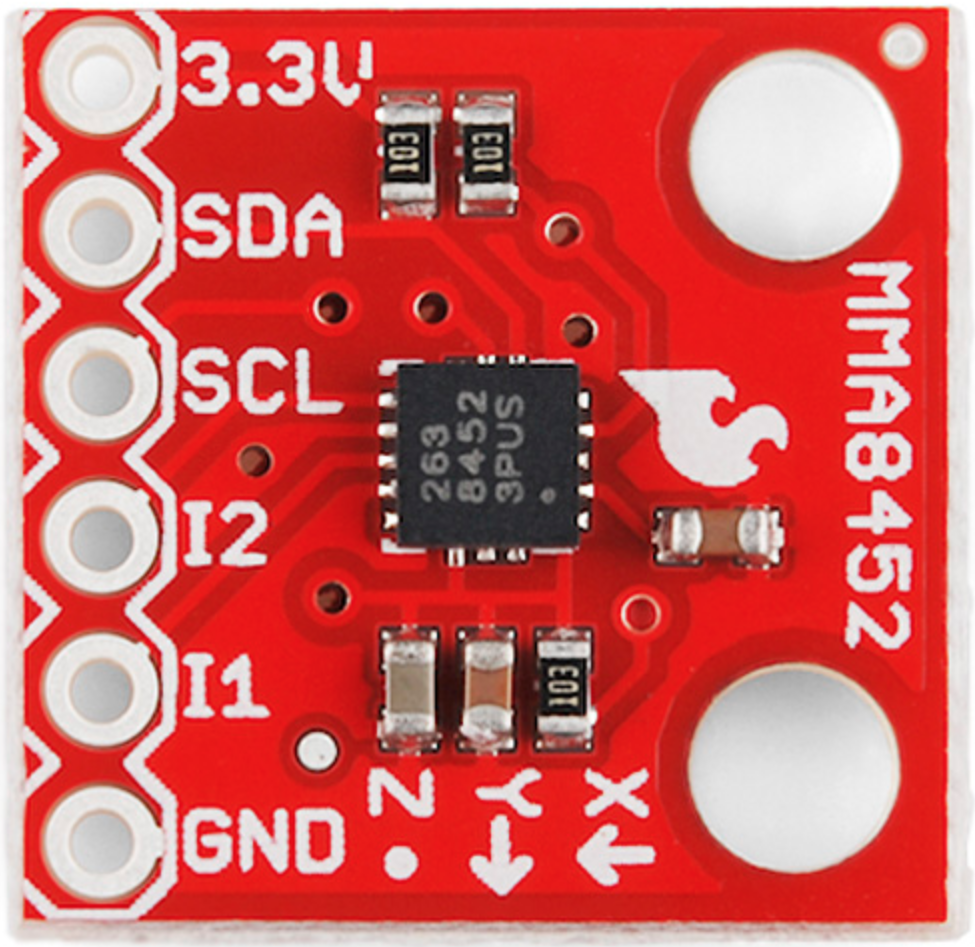
\includegraphics[width=\linewidth]{IMUocean.png}
    \vspace{-8pt}
    {\tiny{Source: \\ Oceancontrols}}
\end{wrapfigure}

%\bigskip
 We propose methods for human physical activity recognition using time series, collected from a  tri-axial accelerometer and gyroscope of a wearable device. Methods solve the problems of time series segmentation, feature extraction and user state classification. We assume that each meaningful segment corresponds to one fundamental period of motion. To perform an adequate behavioral analysis we represent time as a hierarchical structure. It splits a motion, an action, and a process.  

}

\headerbox{Behavioral analysis framework
}{name=rightpanel,column=2,row=0, span=1}{

\medskip
Behavioral analysis outcomes:
\begin{enumerate}[1)]\compresslist
    \item sequential daily classification on hierarchically-segmented time scale,
    \item forecasting of user behaviour and user state alarming,
    \item correction and specification of user GPS position under condition of weak satellite signal.
\end{enumerate}

\vspace{2pt}
The problem is to process time series in high dimensions under small resources of wearable devices.
}

\headerbox{Tri-axial accelerometer sources}{name=triaxial,column=0,below=intro,span=1}{
Our purpose is to perform human
physical activity recognition using data, collected from the built-in tri-axial accelerometer of a mobile phone. This data represents quasiperiodic time series corresponding to one of performed activities: walking, jogging, stair climbing, sitting or standing. For each time series we have to detect the correspondent activity type~\cite{Ignatov2015Accel,Isachenko2018Optima}.

\vspace{-3pt}
\begin{center}
    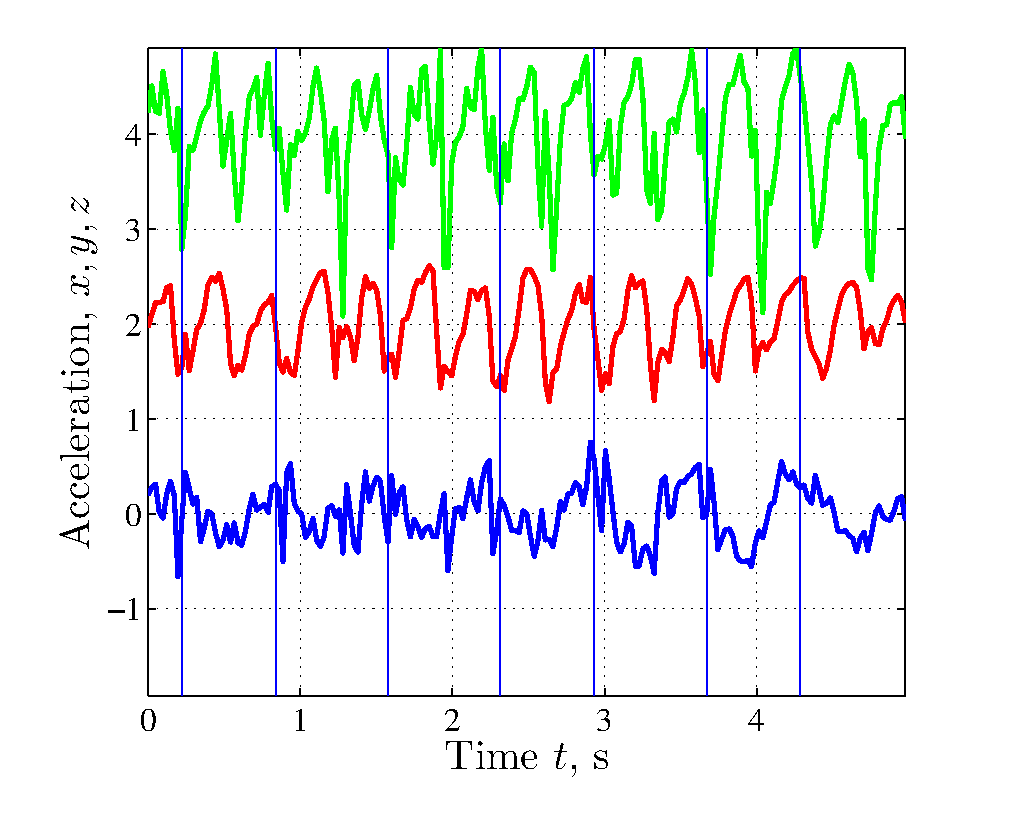
\includegraphics[width=\linewidth]{skipping}
\end{center}
}

\headerbox{Physical activity analysis is based on hierarchical time representation}{name=physical,span=2,column=1,below=intro}{ 
%\vspace{-5pt}
\begin{center}
    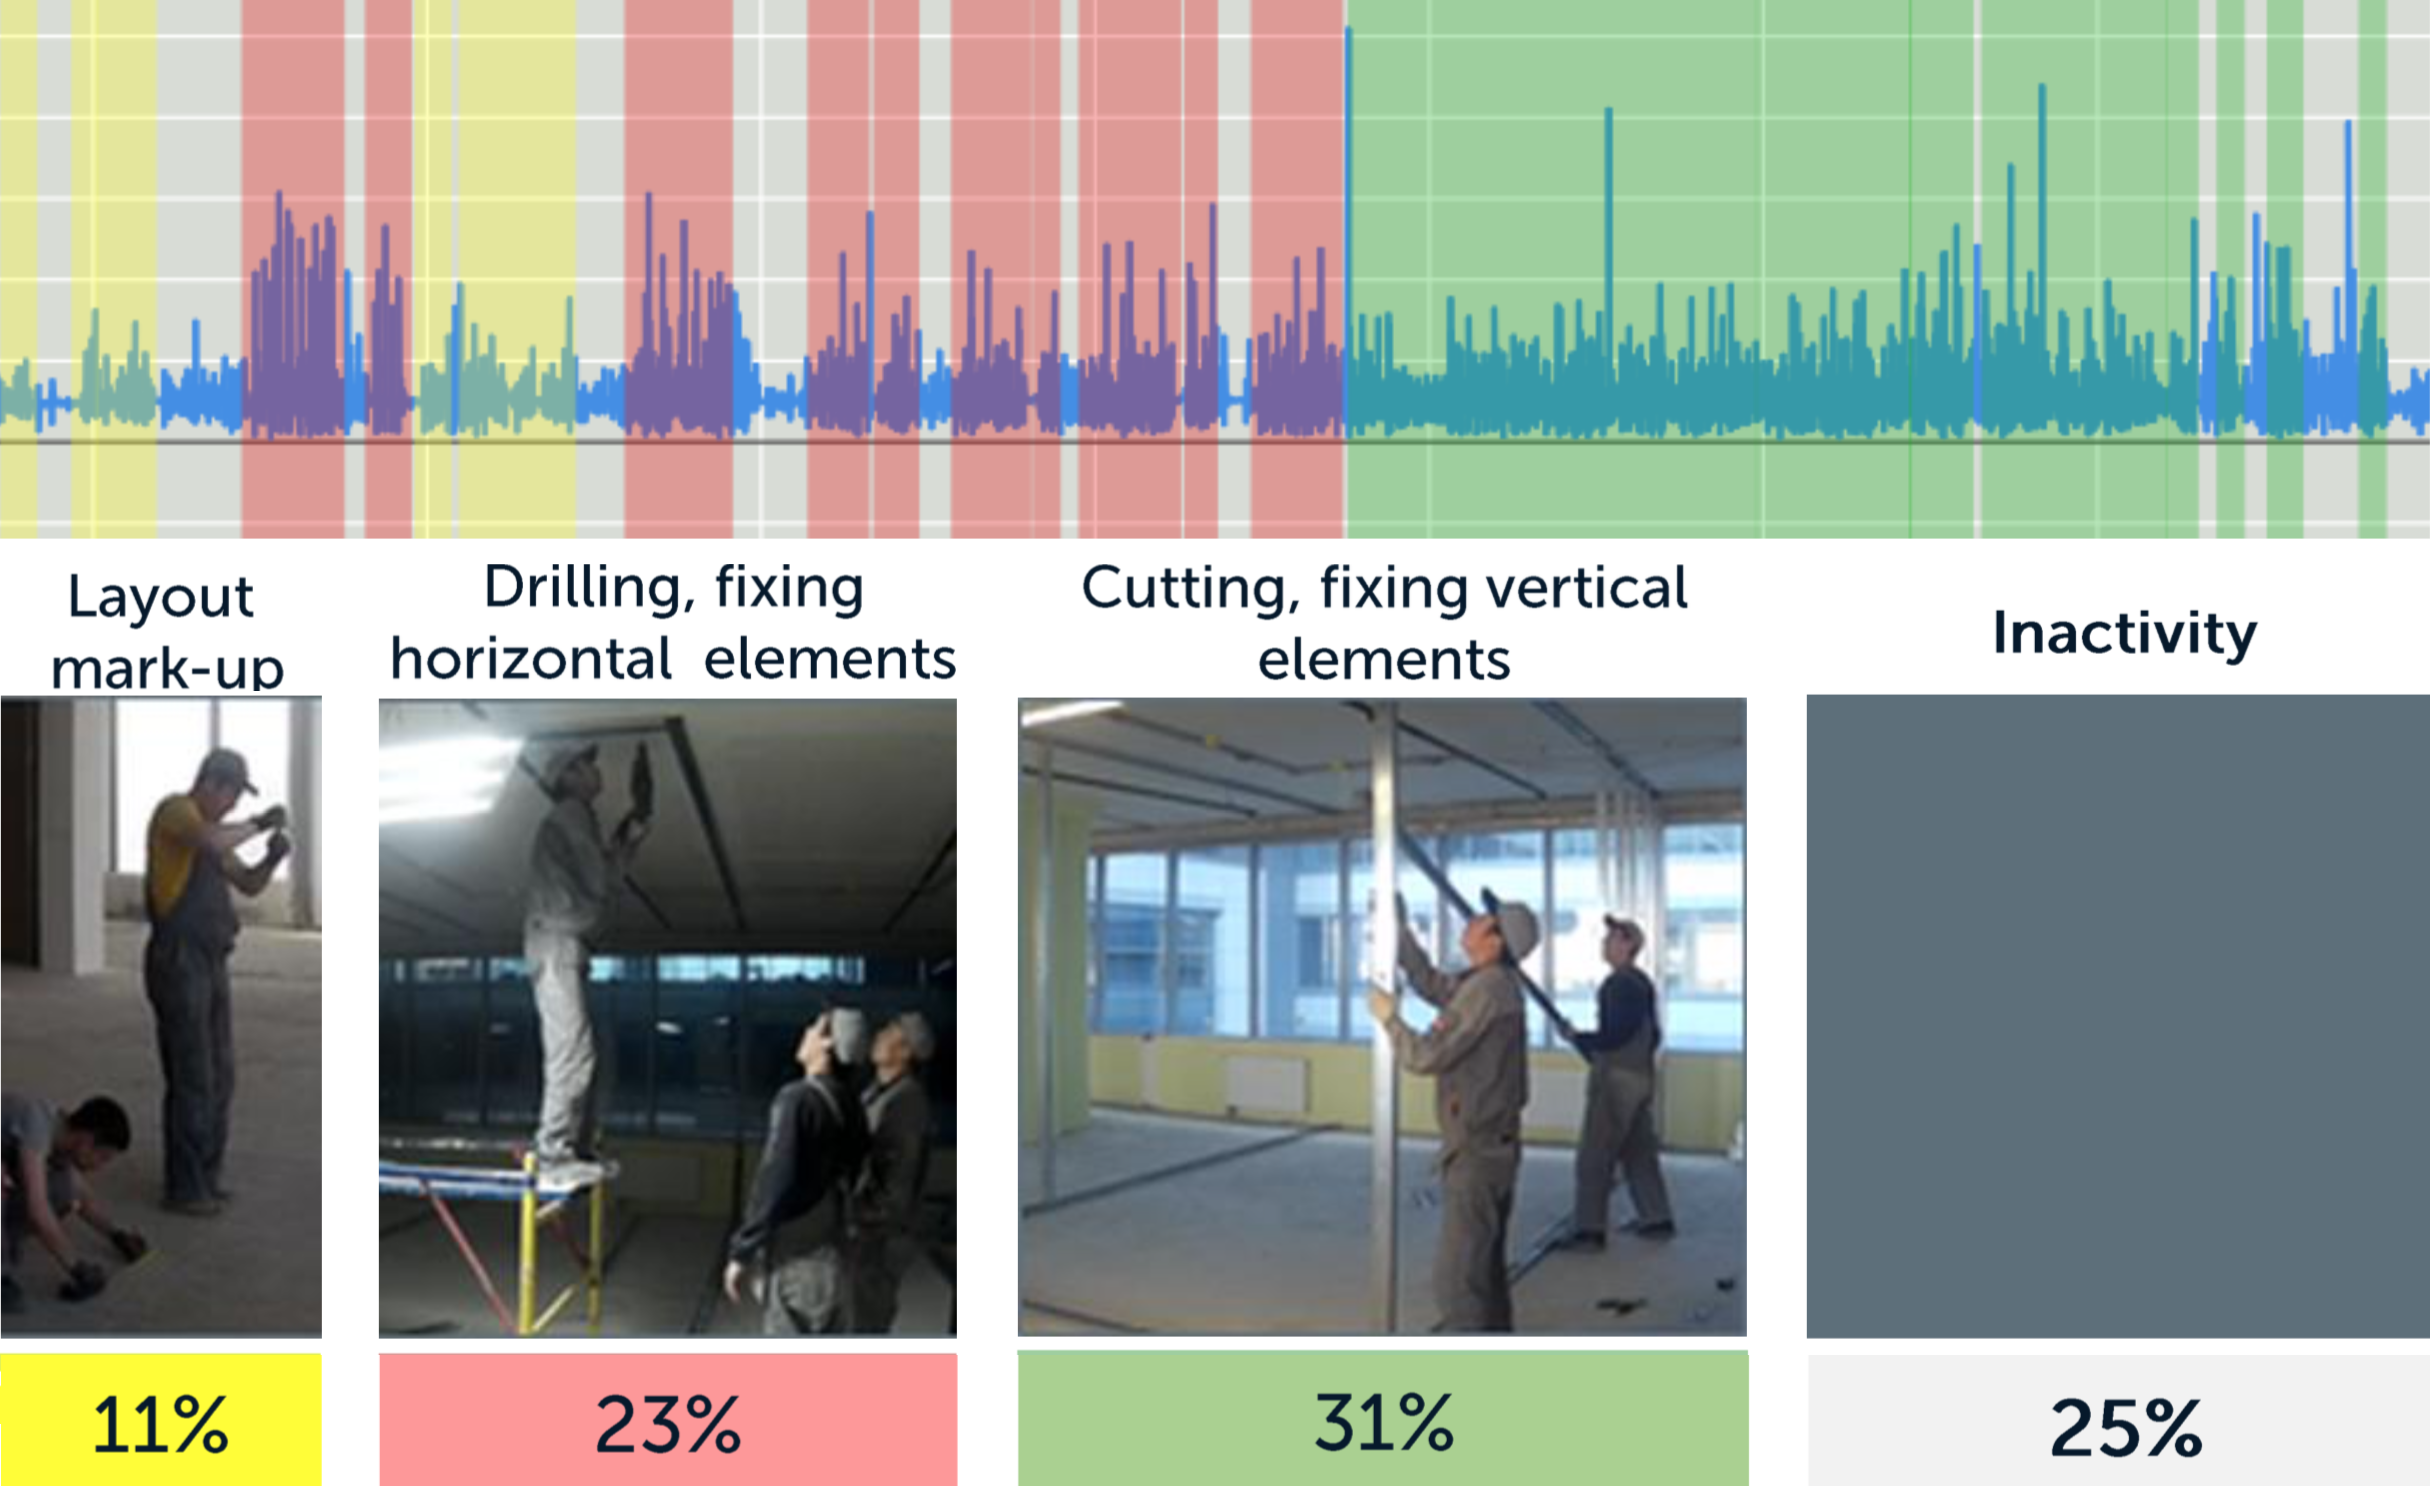
\includegraphics[width=\linewidth]{IMUday2}
\end{center}

\vspace{-9.8cm}
\hfill By courtesy of Forecsys.ru
}

\headerbox{Extracting fundamental periods}{name=extracting,column=0,below=triaxial,span=2}{
We introduce a new definition of nearly periodic time series via triplets $\langle$\emph{basic shape, shape transformation, time scaling}$\rangle$ that covers a wide range of time series. To split the time series into periods we select a pair of principal components of the trajectory matrix. We cut the trajectory of the selected principal components by its symmetry axis,  obtaining half-periods to merge into segments~\cite{Motrenko2016Periods}.
%\vspace{-3pt}

\begin{center}
%    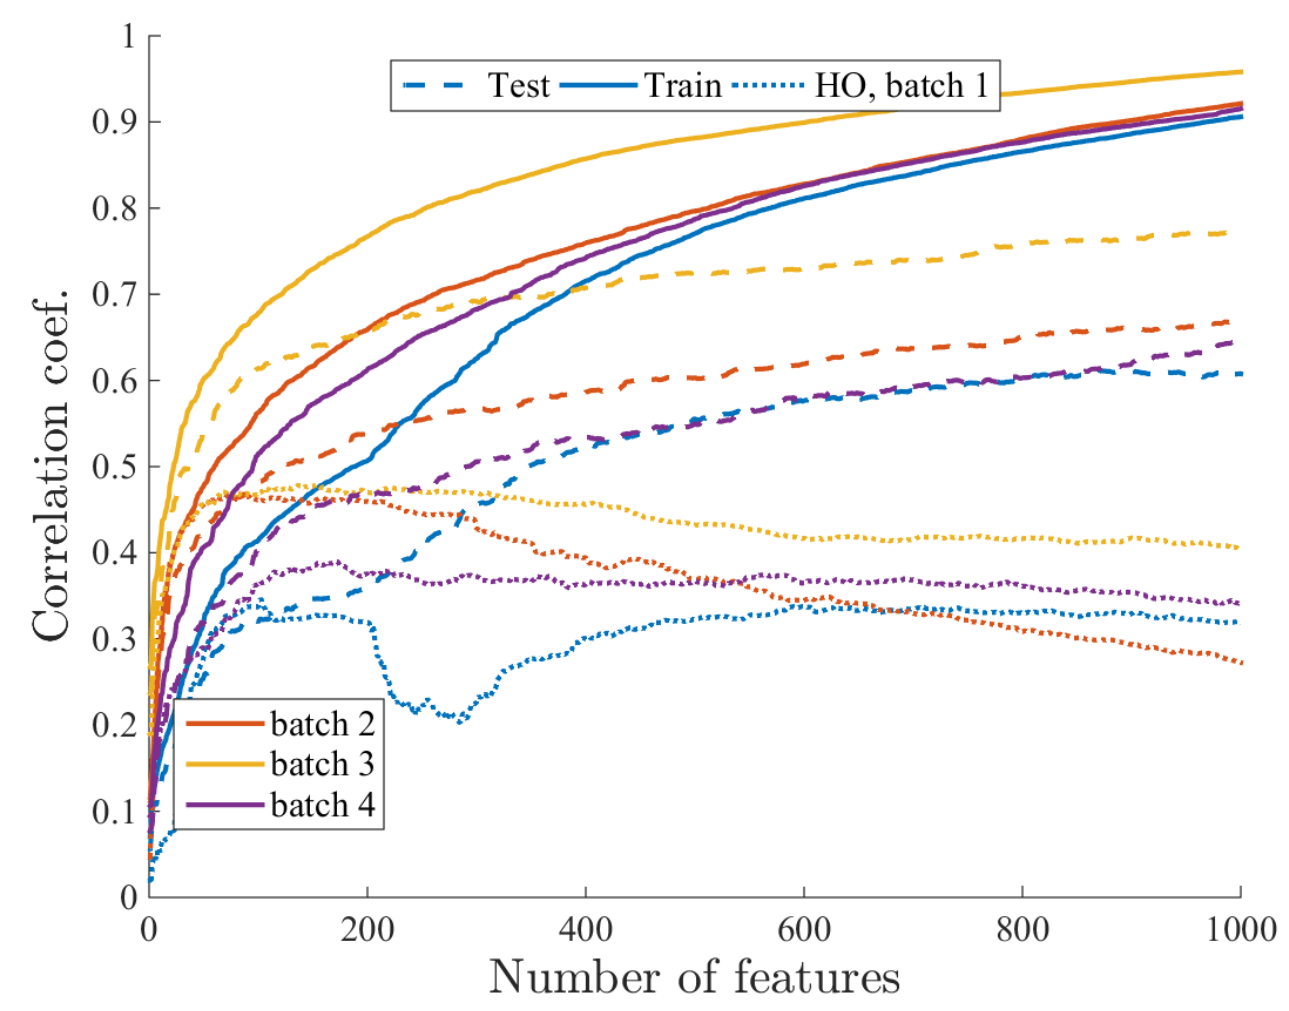
\includegraphics[width=\linewidth]{ECoGQuality.png}
    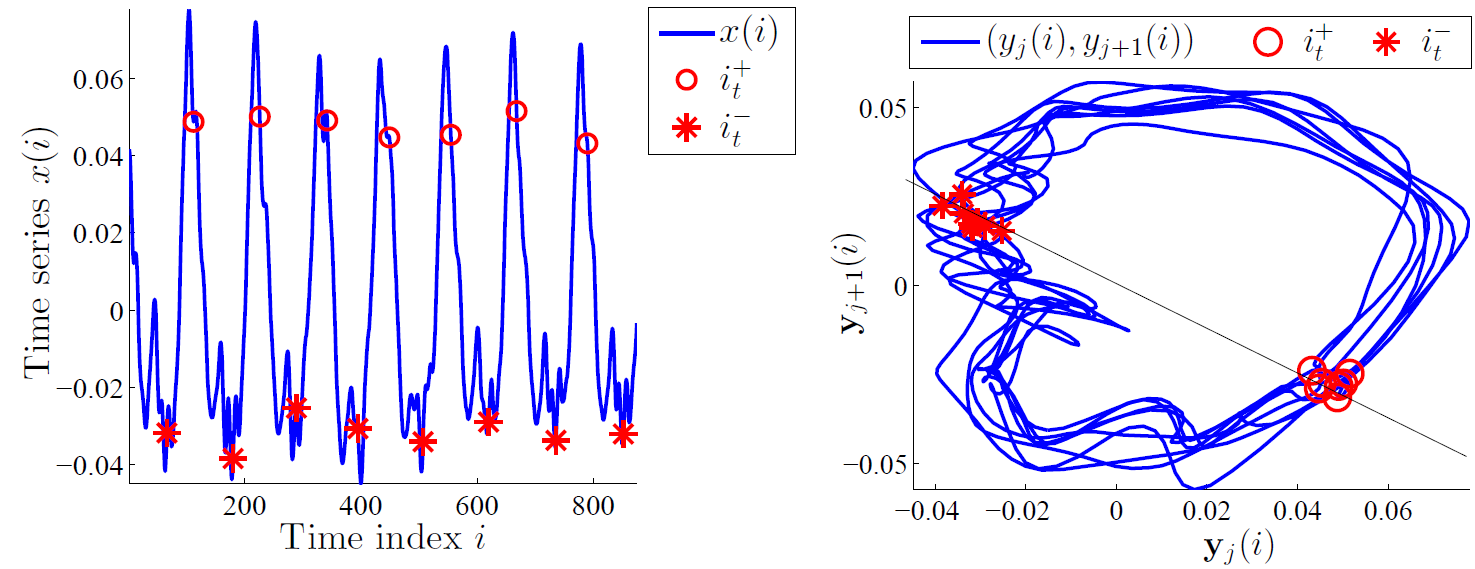
\includegraphics[width=\linewidth]{segmentation}
%\vspace{-4pt}
~~~~~~~~~~~~ Quasi-periodic time series ~~~~~~~~~~~~~~~~~~~~~~~~~ Phase trajectory to set stable periods
\end{center}
}

\headerbox{Performance of  classification}{name=performance,span=1,column=2,below=triaxial}{ 
Feature-based
approach that uses meaningful and concise representations for feature space construction
is applied. The time-series %is considered as a sequence of segments, 
approximated by parametric models and their parameters are used as time-series features. 
\begin{center}
    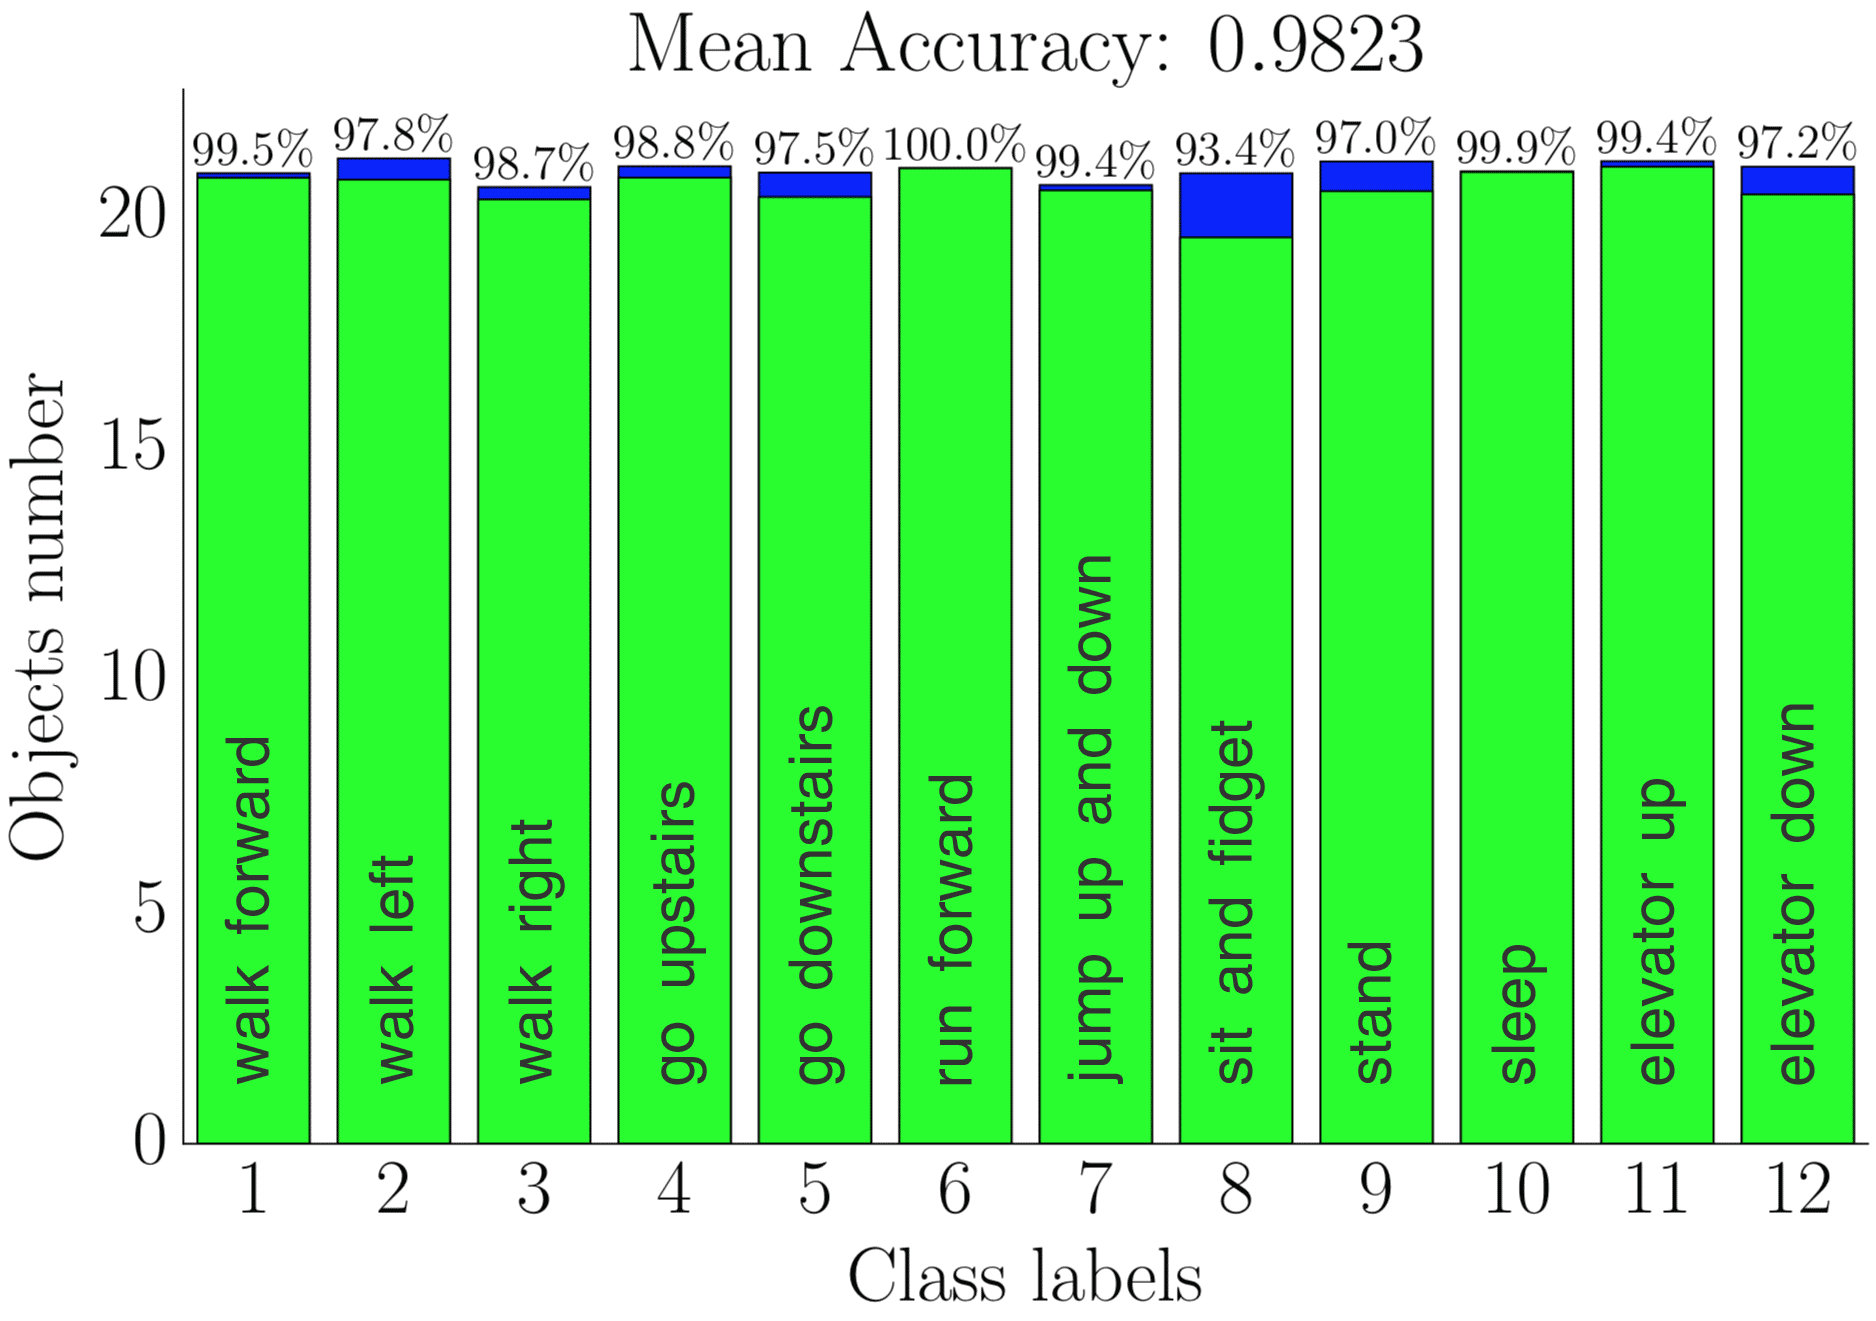
\includegraphics[width=\linewidth]{accel}
\end{center}

\vspace{-0.2cm}
Performance of the human physical activities classification on USC-HAD dataset~\cite{Karas2016Feature}.
}

\headerbox{References}{name=references,column=0,span=3,below=extracting,above=bottom}{
{\footnotesize
\renewcommand{\baselinestretch}{0.6}% Reduce the font size in this block
\renewcommand{\section}[2]{\vskip 0.05em} % Get rid of the default "References" section title
\nocite{*} % Insert publications even if they are not cited in the poster
\bibliographystyle{unsrt}
\bibliography{Motrenko2018IMUposter} % Use sample.bib as the bibliography file
}}
\end{poster}
\end{document}
